\section{Related Works}
\subsection{Generalized AI-Generated Image Detection}
    Generalized AIGI detection seeks to train a model that can generalize to unseen generative model from a single training source. The primary approach can be divided into two categories. The first category is to extract a low-level artifact pattern, and detection is via recognizing this artifact pattern. This generalized pattern is from different domains, including data augmentation \cite{wang2020cnn} and local pixel dependency \cite{tan2024rethinking, liang2025ferretnet} in the common RGB domain. In frequency domain, high frequency component is widely used \cite{tan2024frequency, li2025improving, bihpf}, other domains like reconstruction error \cite{wang2023dire, luo2024lare} and VAE introduced artifact \cite{chen2025dda,rajan2025aligned, liu2025beyond} prove that AIGI artifacts widely exist. The second is through semantic-level artifact, based on the fact that generative models often fail to maintain semantic consistency, which can be detected via a pretrained image encoder. UniFD \cite{ojha2023towards} first explored this direction using a frozen CLIP image encoder. Following works exploit the ability of pretrained encoders in AIGI detection via inserting adapter in CLIP \cite{liu2024forgery, li2025towards} , creating tunable subspace \cite{yan2024orthogonal, zhang2025towards, liu2026mirror}, injecting forgery concept \cite{tan2025c2p} and extract hybrid feature for detection \cite{cheng2025co, yan2024sanity}. However, these detectors often fail to maintain consistency performance under domain gap due to the fingerprint or inconsistency they aim to extract does not appear in all generative models.
    
    
\subsection{Curated datasets for AIGI Detection}

    Existed AIGI detectors were trained on a paired dataset, usually comprise of only one generator or one with its variant \cite{wang2020cnn,chen2024drct, Guillaro2024biasfree,chen2025dda}. To address the generalization challenges, some efforts have begun attempting the use of data from a more diverse source \cite{yang2025d3, yan2024sanity, wen2025spot} to build a more convincing detector. However, their approach to curate the dataset is just simply concatenate the existing datasets, which still lacks breadth and diversity. On the other hand, a series of work recognizes the importance of generator diversity, focusing on building large-scale datasets. Specifically, RED series \cite{red116, red140} curated datasets from hundreds of generators, while Community Forensics \cite{park2025commfor} expanded this to the thousand-generator level. These works still leaves a gap: they are either aimed at tasks other than AIGI detection \cite{red116, red140}, or they train a detector \cite{park2025commfor} with common vision architecture without specialized design to effectively utilize heterogeneous data. To our knowledge, we are the first to simultaneously consider both model-level and data-level challenges in AIGI detection. 
   
\section{Scaling-up AIGI Detectors}

    In this section, we will delve into the paradox of \textbf{\textit{Benefit then conflict}}, explain how it occurs in scaling up settings in a qualitative way and introduce how the proposed GAPL solves the challenges. 
    
%-------------------------------------------------------------------------
\subsection{Challenges in Scaling Up Setting}  
    \label{}
    A common AIGI detector works in the following way. We denote a paired dataset $\mathcal{D}=\{\mathcal{X}, \mathcal{Y}\}$ , where $\mathcal{X}$ is the images set $\mathcal{X}=\{ x_{1}, x_2, ...x_n\}, x_i \in \mathbb{R}^{3 \times H \times W} $ with corresponding label $\mathcal{Y}=\{y_0, y_1, ..., y_n \}, y_i=\{ 0,1 \}$.
    
    To avoid overfitting, common approach \cite{ojha2023towards, yang2025d3} uses an pretrained encoder to extract image embedding $f_i = \phi(x_i) \in \mathbb{R}^D$ , where $ \phi( \cdot ) $ denotes image encoder, and the image embedding refer to its [CLS] token. Subsequently, a classifier $\mathcal{G}$ is applied to predict its log-likelihood, with its parameter $\theta$ optimized via cross entropy loss on dataset $D$:
    \begin{equation}
    \begin{aligned}
       \hat{y} =  & \mathcal{G}_\theta \left( f \right) ,  \\
       \theta = \mathop{\arg\min}_\theta 
       \mathbb{E}_{(x, y) \in D} \Big[
          - \big( & y \log(\hat{y}) + (1-y)\log(1-\hat{y}) \big)
       \Big].
    \end{aligned}
    \end{equation}

    \textbf{Scaling up data itself causes increasing heterogeneity}. The discrepancy in the capacity of generative models to approximate the true distribution leads to an increased variance in the combined distribution of different generative models. We consider a dataset distributed according to a gaussian mixture, a series of generative models fit this distribution by maximizing likelihood on this dataset: 
    \begin{equation}
        \begin{aligned}
            \{x|(x,0)\} \sim P_{real} &=\sum_{k}^{K}\pi_k \mathcal{N}(\mu_k, \Sigma_k) \\
            \{x|(x,1)\} \sim P_{gen} &=\sum_{i}^{G}w_i\sum_{j}^{K}\pi_{i,j}\mathcal{N}(\mu_{i,j},\Sigma_{i,j}),
        \end{aligned}
    \end{equation}
    then, according to the law of total variance, the covariance matrix can be calculated with:
    \begin{equation}
        \begin{aligned}
            \Sigma_{real} & = \mathbb{E}(\Sigma)+\text{Var}(\mu), \\
            \Sigma_{gen} & = \mathbb{E}_G \left[ \text{Var}(X |G) \right] + \text{Var} _G\left[ \mathbb{E}(X|G)\right] \\
             &  = \underbrace{\mathbb{E}_M \left[ \text{Var}(X|G_i,M)|G_i\right]+\text{Var}_M\left[\mathbb{E}(X|G_i,M)|G_i \right]}_{\text{generator fitting variance}} \\
             & + \underbrace{\text{Var}_G \left[ \mathbb{E}(X|G)\right]}_{\text{cross generator variance}},
        \end{aligned}
    \end{equation}
    where $M$ denotes mode in GMM. The first two terms reflect variance in the learned distribution, which correspond to the terms of the real covariance. The third term, reflects cross generator variance which grows as generator diverse.
    
    To validate our proposal, we conducted an experiment where we collected a series of datasets from GenImage \cite{zhu2024genimage}. In each dataset, there are a total number of 8,000 images from ImageNet \cite{imagenet} and the same number of images generated with several models trained on ImageNet, with the number of models varying from 1 to 8. We also uses a dataset with thousands of generative models to further provide large scale setting. For detailed information of these datasets and our experiment, please refer to Appendix.\ref{sec:pre-exp}.   To estimate the heterogeneity in the dataset, we use scatter matrix of image feature as a proxy for covariance matrix $\Sigma$. For a set $C$, its scatter matrix is calculated by:
    
    \begin{equation}
        S = \sum_{f \in C} \left( f-\mu \right) \left( f-\mu\right)^T,
    \end{equation}
    where $\mu=\frac{1}{N}\sum f$ is the mean feature of the extracted features in this set. We calculate the trace of this scatter matrix $tr(S)$ to evaluate total variance of real and generated images.

    Results are presented Fig.~\ref{fig:stat} (a). The figure illustrates that: for the first four datasets, the variance of the generated images exhibits a clear upward trend that scales with the number of generators. Conversely,  the variance of real images is highly consistent. In the last dataset, which incorporates real and generated images from diverse sources,  the variance of the generated distribution is still markedly higher than that of the real distribution. This confirms our hypothesis: the heterogeneity of real images remain stable whereas the heterogeneity of generated images increases as more generators are introduced. 

    \begin{figure}[!tp]
        \centering
        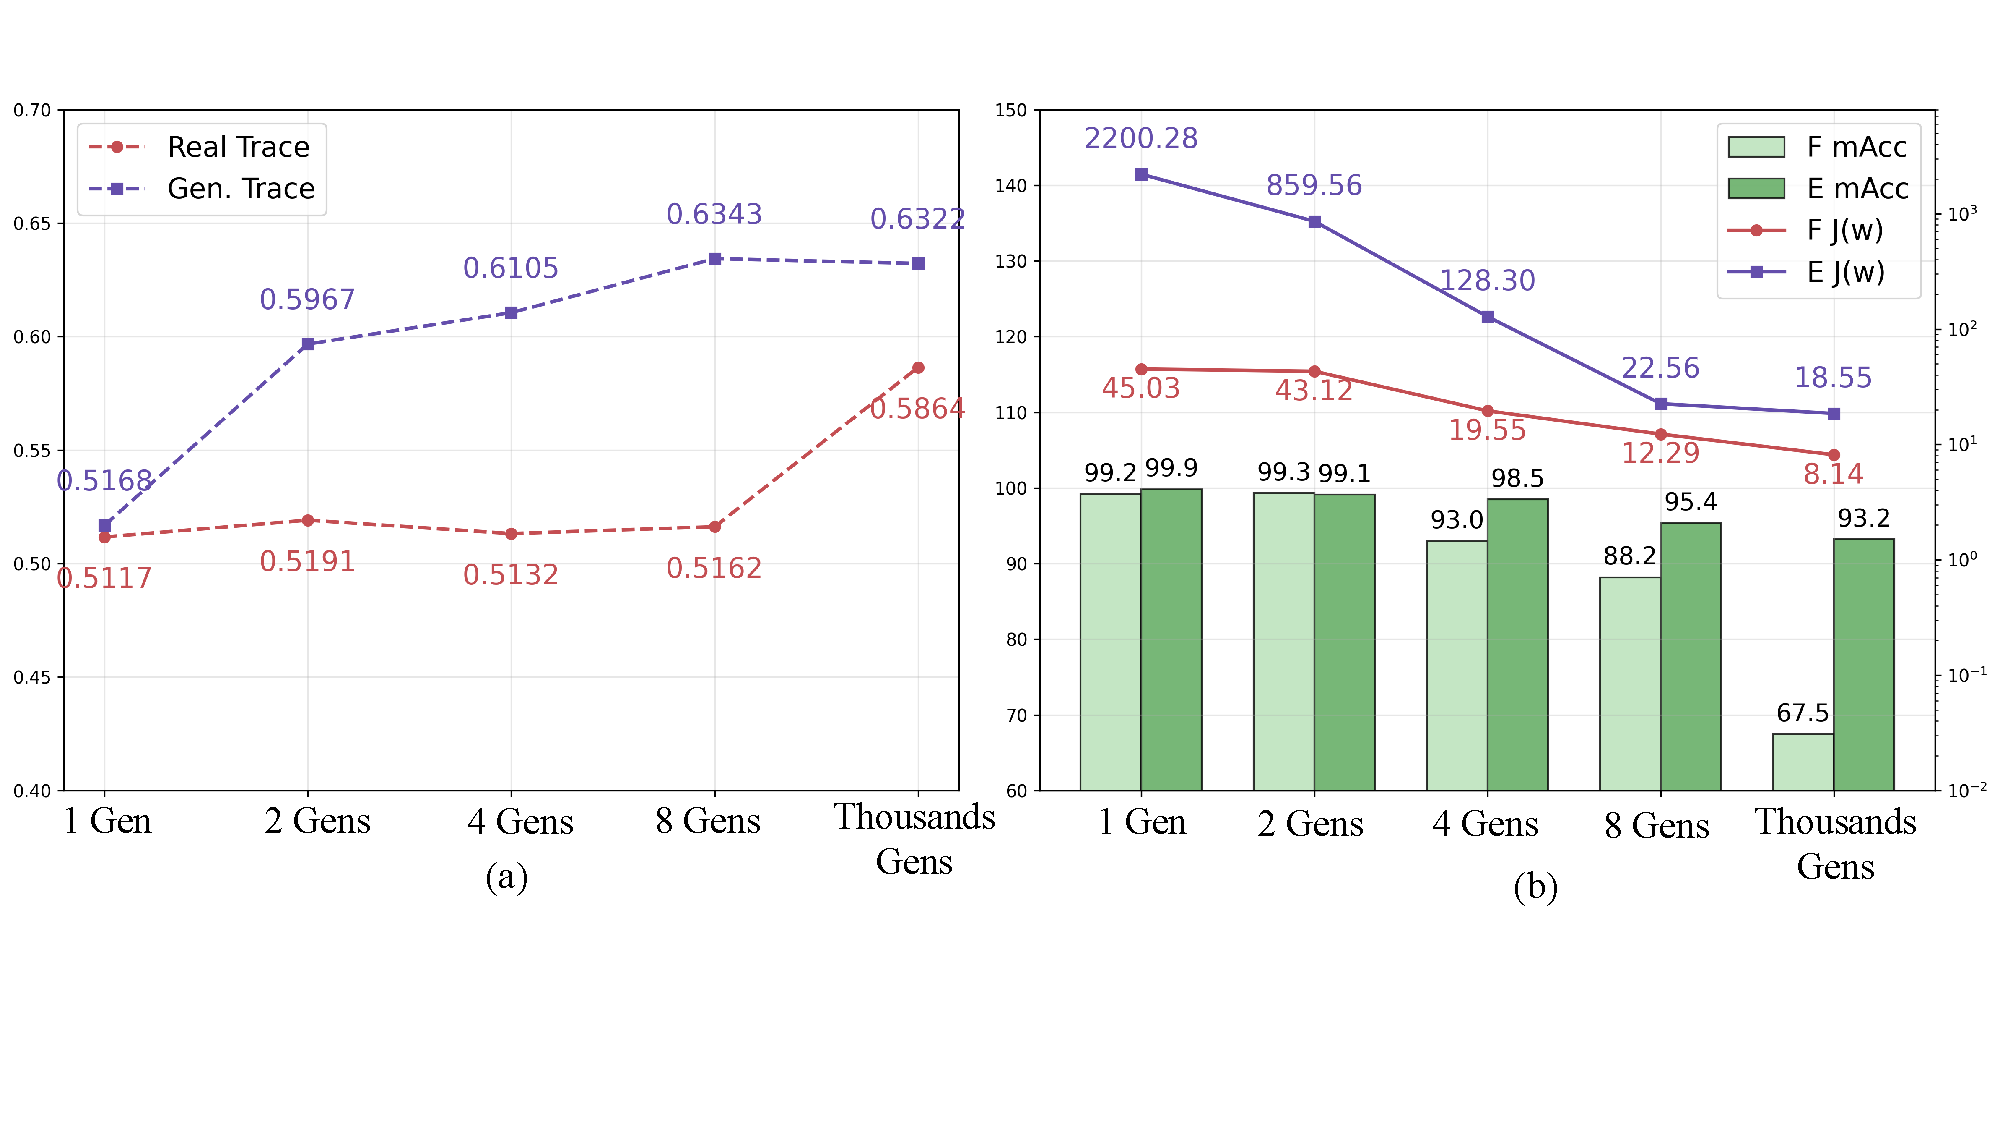
\includegraphics[width=\linewidth]{figs/stat.pdf}
        \caption{Results of the experiment on a series of datasets comprise of different number of generators.  \textbf{(a)} Trace of the scatter matrix from generated images is significantly higher than that from real images.  \textbf{(b)}  Accuracy of validation and \textit{Fisher ratio $J$} between end-to-end ($\mathbf{E}$) and frozen-encoder models ($\mathbf{F}$), end-to-end models tend to have a higher separability and accuracy, especially in scaling up settings. ``Gen(s)'' denotes ``Generator(s)''. } 
        \label{fig:stat}
    \end{figure}
    
    \textbf{Reliance on a frozen encoder sets bottleneck to model performance}.
        Common AIGI detectors leverage a pre-trained encoder to avoid overfitting and enhance generalization, This dependency indicates that when training images on novel generators, the model can only push their representations towards the real or generated classes in the feature space, rather than learning the new generative artifacts. This often results in a poor decision boundary and lower discriminability. To investigate the intrinsic discriminability of the feature space, we analyze the embeddings using Linear Discriminant Analysis (LDA) \cite{fisher1936use}. LDA seeks to create a linear projection space and provides  a quantitative measure \textit{Fisher ratio} of this class separability, allowing us to assess how well the pre-trained embeddings can inherently distinguish between real and generated images. Moreover, its optimization can be given in closed form:
        
    \begin{equation}
        \begin{split}
          w & = \mathop{\arg\max}_{w}J (w)=\frac{w^TS_bw}{w^TS_ww} \\
            & =  kS_{w}^{-1}\left( \mu_0-\mu_1 \right),
        \end{split}
    \label{eq:ldaoptim}
    \end{equation}
    where $S_b, S_w$ are scatter between classes and within class matrices, respectively, which can be calculated by
    \begin{equation}
        \begin{split}        
            & S_w = \sum_{i=0}^{C}S_i \\ 
            & S_b = (\mu_0-\mu_1)(\mu_0-\mu_1)^T
        \end{split}
    \label{eq:ldas}
    \end{equation}
        We designed an experiment with the datasets introduced above in the following steps: (1) For each dataset, train an end-to-end classifier, simultaneously, train a classification head based on an frozen image encoder of CLIP. (2) Extract penultimate representation from the two models on validation set, estimate $J$ based on eqs.~\eqref{eq:ldaoptim} and \eqref{eq:ldas} and classify them with a threshold of 0.5. We report detection accuracy and \textit{Fisher ratio} $J$ as metrics.

        The results are presented in Fig.~\ref{fig:stat}(b). Results reveal that first,  \textit{Fisher ratio} and detection accuracy drops as more diverse data adds. Second, an end-to-end detector has a higher \textit{Fisher ratio} on the same data scale compared to the pretrained-based one. Although they achieve good generalization by training on single source with a relatively small \textit{Fisher ratio}, they seemed to be indistinguishable to more generators. This lead us to reflect that the reliance of pretrained encoder in prevalent AIGI detectors may fundamentally impose an upper bound on achievable performance when scaling up AIGI detection. 
        


%-------------------------------------------------------------------------
\subsection{Scaling Up with Generator-Aware Prototypes}
    \begin{figure*}[!tp]
        \centering
        
\includegraphics[width=1.0\linewidth]{figs/overview.pdf}
        \caption{\textbf{The overall framework of our GAPL.} We train the GAPL in two stages. In the first stage, we train a MLP and extract embeddings for PCA decomposition, we only retain top $N$ components as prototypes; in the second stage, we uses LoRA to finetune the encoder and map image embedding to prototypes to get the final logits. }
        \label{fig:method}
        % \vspace{-0.1in}
    \end{figure*}
    Up to now, we have identified key challenges in building a scaling up AIGI detector:  (1) To lower inner heterogeneity of generated images, we need to achieve a compact representation for the generated images. (2) Fixed embedding space should be abandoned. Relying on a static embedding space like a frozen CLIP is fundamentally limiting. 
    
    To tackle the two challenges, we propose GAPL for scaling up AIGI detection. we adopt a philosophy called \textit{Turn Thousand into a Few}, the GAPL learns a compact shared prototype space to distill thousands of generators into a few, representative prototypes. This process is via a two-stage learning framework, we first leverage pretrained encoder to construct prototype, then we let prototypes guide the encoder to learn and project to this prototype space. The framework of  GAPL is shown in Fig.~\ref{fig:method}.

\textbf{STAGE I: Creating Forensic-Realated Space and Generator-Aware Prototypes.}
   
    The objective of this stage is to perform a supervised projection, creating a forgery-related subspace based on the pretrained embedding space. Since most pretrained encoder are highly correlated with semantic information due to its pretraining objective, we aim to endow the encoder with a basic understanding of generated images, enabling it to capture representative concepts. 
    
    Specifically, We select an amount of $M$ images each from ProGAN\cite{karras2018progressive}, Stable Diffusion v1.4 \cite{rombach2022high}, and Midjourney \cite{Midjourney}, sourced from the ForenSynths \cite{wang2020cnn} and GenImage \cite{zhu2024genimage} as they represent GANs, Latent diffusion models and Commercial APIs to form a prototype set. We also pair the same amount of real images accordingly. Then, an MLP was attached after the encoder to project dimension and get logits for classification, the projection and MLP can be formulated with $g_{proj}: \mathbb{R}^{D} \xrightarrow{} \mathbb{R}^{D'}$ and $\texttt{MLP}: \mathbb{R}^{D} \xrightarrow{} \mathbb{R} $. This process can be formulated as follow:
    \begin{equation}
        \begin{split}
            & f = \phi(x),  \\
            & \hat{y} =\texttt{MLP}\left(\texttt{Normalize}(f) \right),
        \end{split}
    \end{equation}
    where $\phi(\cdot)$ is the image encoder. In the first stage, the image encoder keeps frozen, we only train this MLP with binary crossentropy as loss function on the prototype set.
    
    Subsequently, we utilize the intermediate layer of the MLP to extract forgery-related embeddings to build prototypes. $\mathbf{F}_f = [f_1^f, f_2^f,  ..., f_{M \times 3}^f]$ , $\mathbf{F}_r = [f_1^r, f_2^r,  ..., f_{M \times 3}^r]$, $f \in \mathbb{R}^{D'}$, denotes the real and generated subset of these embeddings. We then perform principle component analysis (PCA) separately on the two subsets for prototype constructing, and select the top $N/2$ principal components from each subset as Generator-Aware Prototypes:
    \begin{equation}
    \begin{split}
            C = \frac{1}{3M - 1} \left( \mathbf{F}_f - \mathbf{1}\mathbf{\bar{\mu}} \right)^T &\left( \mathbf{F}_f - \mathbf{1}\mathbf{\bar{\mu}} \right), \\
            Cv_i=\lambda_iv_i, \\
        \mathbf{P_f}= \left[ v_1, v_2, ..., v_{N/2} \right]^T & \in \mathbb{R}^{(N/2) \times D'},
    \end{split}
    \end{equation}
    where $\bar{\mu} \in \mathbb{R}^{1 \times D'}$ is mean vector of the embeddings in $\mathbf{F}$. $\mathbf{1}^T_{3M} \in \mathbb{R}^{3M}$ denotes all-one vector. We concatenate real and generated prototypes to form the final prototype matrix $\mathbf{P}=[\mathbf{P_r}; \mathbf{P_f}] \in \mathbb{R}^{N \times D'} \ $.
    
    We adopt this selection strategy based on the assumption that, PCA decomposes the covariance matrix, the components with larger variance capture more general forgery-related information, while those with smaller variance reflect generator-specific characteristics. The remaining components, which contribute little to the overall variance, are mainly task-irrelevant noise and thus discarded. 
    
\textbf{STAGE II: Map Generators to Prototypes for Large Scale AIGI Detection.}
   In the second stage, we further enhance the model's capability, adhering to our principle of not relying on a fixed embedding space. To maintain as much knowledge as possible in pretrained image encoder, this adaptation is performed using LoRA \cite{hu2022lora}.
   
    \begin{equation}
        f=g_{proj}\left( \phi_{lora}(x) \right).
    \end{equation}
        
  Furthermore, we aim to solve how to effectively integrate the extracted prototype with the image feature from image encoder. Given that our primary objective is to enforce feature in a low variance way, we posit that a good approach is to represent each image's features into a dynamic linear combination of these learned prototypes. It should create a map from the diverse feature space onto a low-variance prototype space. Therefore, we adopt a simple yet effective cross-attention \cite{vaswani2017attention} mechanism as this mapping to perform feature fusion, where the image embedding act as queries and the prototypes serve as keys and values. It can be expressed as follows: 
\begin{equation}
 \begin{split}
    \tilde{f} & = \texttt{Attn} \left(W_qf, W_k\mathbf{P}, W_v\textbf{P} \right) \\
      & =  softmax(\frac{(fW_q)(\mathbf{P}W_k)^T}{\sqrt{D'}}) \cdot \mathbf{P}W_v 
 \end{split}
 \end{equation}

    Where $W_q,W_k,W_v \in \mathbb{R}^{D' \times D'}$ is the respective affine matrix. We feed this re-organized feature $ \tilde{f} $ into a linear classifier to predict its final logits and train the whole model with binary crossentropy.

\begin{table*}[h]
\centering
\renewcommand{\arraystretch}{1.1}
\resizebox{\textwidth}{!}{
\begin{tabular}{l l cc cc cc cc cc cc cc}
\toprule
\multirow{2}{*}{\textbf{Method}} & \multirow{2}{*}{\makecell{\textbf{Training}\\\textbf{Class/Num.}}} &
\multicolumn{2}{c}{\textbf{ForenSynths}} & \multicolumn{2}{c}{\textbf{UFD}} & \multicolumn{2}{c}{\textbf{GenImage}}  & \multicolumn{2}{c}{\textbf{SynthBuster}} & \multicolumn{2}{c}{\textbf{Chameleon}} & \multicolumn{2}{c}{\textbf{CommFor}} & \multicolumn{2}{c}{\textbf{Mean}} \\
\cmidrule(lr){3-4} \cmidrule(lr){5-6} \cmidrule(lr){7-8} \cmidrule(lr){9-10} \cmidrule(lr){11-12} \cmidrule(lr){13-14} \cmidrule(lr){15-16}
 &  & Acc & AP & Acc & AP & Acc & AP & Acc & AP & Acc & AP & Acc & AP & Acc & AP \\
\midrule
\multicolumn{16}{l}{\cellcolor{gray!25}\textit{GAN-Generalized}} \\
\midrule
CNNDet \cite{wang2020cnn} & ProGAN/720k & 75.3 & 91.8 & 53.1 & 71.1 & 51.3 & 65.6 & 50.3 &  53.9 & 57.0 & 42.6  & 51.5 & 53.7 & 56.4 & 63.1 \\
NPR \cite{tan2024rethinking}  & ProGAN/144k & 90.8 & 91.8 & 95.1 & 97.4 & 86.2 & 91.6 & 38.9 & 45.4 & 57.4 & 47.7 & 73.8 & 74.7 & 73.7 & 74.8 \\
UniFD \cite{ojha2023towards} & ProGAN/720k & 89.4 & 96.7 & 82.2 & 95.7 & 70.0 & 88.3 & 67.6 & 78.0 & 57.2 & 46.2 & 54.0 & 58.3 & 70.1 & 77.2  \\
SAFE \cite{li2025improving} & ProGAN/144k & \underline{96.2} & \underline{98.6} & 95.7 & 99.1 &  95.5 & 99.3 & 44.7 & 44.7 & 59.2 & 50.6 & 50.0 & 48.3 & 73.6 & 79.2 \\
AIDE \cite{yan2024sanity} & ProGAN/720k & 88.4 & 96.0 & 96.7 & 99.0 & 92.0 & 97.5 & 48.0 & 49.9 & 58.4 & 50.1 & 49.9 & 47.1  & 72.2 & 73.3 \\
\midrule
\multicolumn{16}{l}{\cellcolor{gray!25}\textit{Diffusion-Generalized}} \\
\midrule
DRCT \cite{chen2024drct} & SD2.1/473k & 50.0 & 49.7 & 70.0 & 79.2 & 78.0 & 94.0 & 77.6 & 84.7 & \textbf{79.8} & \textbf{85.2} & 49.6 & 49.4 & 67.5 & 73.7 \\ 
Co-SPY \cite{cheng2025co} & SD1.4/320k & 65.6 & 75.9 & 76.8 & 84.3 & 78.0 & 94.1 & 77.4 & 91.6 & 68.8 & 68.8 & 67.9 & 79.2 & 72.4 & 82.3   \\
B-Free \cite{Guillaro2024biasfree} & SD2.1/360k & 81.1 & 94.2 & 87.1 & 95.3 &  87.3 & 97.7 & \textbf{94.9} & \textbf{98.8} & \underline{78.2} & \underline{85.2} & 81.5 & 91.8 & 85.0 & \underline{93.8} \\
\midrule
\multicolumn{16}{l}{\cellcolor{gray!25}\textit{Scaling-Ups}} \\
\midrule
AIDE \cite{yan2024sanity} & 8gens/1.3M & 85.3 & 93.8 & \textbf{98.5} & \textbf{99.9} & \textbf{99.7} & \textbf{100.0} & 52.7 & 56.0 & 65.8 & 69.7 & 50.1 & 48.2 & 75.4 & 77.9 \\
D3 \cite{yang2025d3} & 9gens/2M & 93.0 & 97.9 & 94.8 & 99.0 & 95.4 & 99.2 & 81.3 & 89.5 & 61.0 & 56.5 & 73.6 & 86.0 & 83.2 & 88.0 \\
% D3^{\dagger}\cite{yang2025d3} &  & 75.1 & 90.4 & 57.0 & 72.2 &  59.1 & 75.3 & 72.2 &  80.5 & 58.1 \\ 
CommForen \cite{park2025commfor} & 4.7Kgens/5M & 92.3 & 98.2 & 94.0 & 97.0 & 84.0 & 93.4 &  87.0 & 94.7 & 77.5 & 83.5 & \underline{86.8} & \underline{93.9} & \underline{86.9} & 93.4 \\
\rowcolor{cvprblue!20}
GAPL(Ours) & 4.7Kgens/550k & \textbf{97.2} & \textbf{99.5} & \underline{97.2} & \underline{99.8} & \underline{96.7} & \underline{99.6} & \underline{91.1} & \underline{97.2} & 71.0 & 75.6 & \textbf{89.4} & \textbf{97.8} & \textbf{90.4} & \textbf{94.9} \\ 
% GAPL(16) & 4.8Kgens/550k & 97.0 & 99.5 & 97.0 & 99.8 & 96.7 & 99.5 & 90.5 & 97.1 & 69.9 & 74.0 \\
\bottomrule
\end{tabular}
}
\caption{Overall performance of different detectors across benchmarks. \textit{GAN-Generalized} means that these models were trained on GAN-generated images, \textit{Diffusion-Generalized} means diffsuion-generated images accordingly. \textit{Scaling-ups} means that these model have the access to all kinds of images. We also report each detector's generator type and number of images of their training set.}
\label{exp1}
\end{table*}


%-------------------------------------------------------------------------
\section{Experiments}

In this section, we evaluate the proposed GAPL to validate the followng \textbf{Reseach Questions (RQs)} :
\begin{itemize}
    \item RQ.1: How well does the proposed \textbf{GAPL} in detecting generated images from any generator?
    \item RQ.2: How well is the inherent potential of proposed \textbf{GAPL} in model architecture?
    \item RQ.3: Why is the designed Prototype Learning and two-stage training useful?
    \item RQ.4: How does the number of prototypes and selection of prototype sets affect performance?
    \item RQ.5: How well is the proposed \textbf{GAPL's} robustness in handling post processing?
\end{itemize}

\subsection{Experiment Details}
    \textbf{Training set.} In our GAPL, prototype set and scaling up set are used for training. In the prototype set used in first stage, we select $M = 2000$ images generated by ProGAN \cite{karras2018progressive}, SDv1.4 \cite{rombach2022high} and Midjourney \cite{Midjourney}. These images are sampled from Forensynths and GenImage. As for scaling up dataset, we choose the Community-Forensic \cite{park2025commfor}. This dataset manually chose 12 GANs, 3 pixel diffusion models and collected about 4000 latent diffusion models on huggingface, constituting a large and diverse datasets that covers most generative architectures. We use a small version, compared to the original dataset of 5.4M images, the small version only contains 550k images while the total number of generative models remains the same.

 \begin{table}[t]
        \centering
        \resizebox{0.48\textwidth}{!}{
        \begin{tabular}{l |c c c}
             \toprule
             Dataset & \#Real/\#Fake & \# Models & Type of models  \\
             \midrule
             ForenSynths \cite{wang2020cnn} & 31k/31k & 8 & GAN \\
             UniversalFakeDetect \cite{ojha2023towards} & 8k/8k &8 & Diffusion \\
             GenImage \cite{zhu2024genimage} & 48k/48k & 8 & GAN\&Diffusion \\
             Synthbuster \cite{synthbuster} & 1k/9k & 9 & Diffusion \\
             Chamelon \cite{yan2024sanity} & 14.9k/11.2k & -  & Unknown \\
             Community-Forensics Eval \cite{park2025commfor} & 25k/25k & 21 & Diffusion \\
             \bottomrule
            \end{tabular}
        }
        \caption{The selected 6 AIGI benchmarks to evaluate the methods.}
        \label{tab:testset}
    \end{table}
    
    \textbf{Testing set.} We select six benchmarks to evaluate our method's generalization, covering a spectrum of common and advanced generative models developed over the last decade. Tab.~\ref{tab:testset} lists some information about the benchmarks. Note that despite the use of a large scale training set, more than half of generative models in testing set are still unseen by the detector. See Appendix.~\ref{sec:benchmark} for detailed introduction of these benchmarks.

    
\textbf{Implementation Details.}
    We use the image encoder of CLIP-ViT:L \cite{CLIP, dosovitskiy2020vit} for finetuning. We select $M=2000$ images each from 3 generators as prototype set, along with the same amount of real images. The dimension of projection is set to be $D'=128$, and the number of prototypes is $N=64$.  The experiment was conducted on 2 GeForce RTX 4090 GPUs. More details are in Appendix.~\ref{sec:impledet}

\subsection{Comprehensive evaluation of detection performance across generators (RQ.1)}
    To evaluate the overall detection performance of the proposed GAPL, we conduct test on the 6 selected benchmarks. The results are shown in Tab.~\ref{exp1}. The results reveal the following: \textit{\textbf{(1) Generalized AIGI detectors fail to maintain performance}}. Generalized detectors can achieve a promising performance on only one or two benchmarks. Detectors like SAFE \cite{li2025improving}, achieve an over 95\% accuracy on the previous 3 benchmarks, but fails on the latter 3 with about 50\% accuracy, which demonstrates that it is hard to build a well generalized detector on one training source. \textit{\textbf{(2) GAPL exhibits consistent and promising performance}.} The proposed GAPL achieves a 90.4\% average accuracy across 55 test subsets in 6 benchmarks, with a 3.5\% average accuracy improvement over the previous detectors. Additionally, we reach a 94.9\% average precision and over 90\% mAP in most benchmarks, which further validates our promising detection against generated images. 

\begin{table}[t]
   \centering
    \renewcommand{\arraystretch}{1.1}
    \resizebox{0.48\textwidth}{!}{
    \begin{tabular}{l| c | c c c c c}
     \toprule
        \textbf{Method} & \textbf{Venue} &\textbf{FS} & \textbf{UFD} & \textbf{GI} & \textbf{SB} & \textbf{Mean} \\
        \midrule
        \multicolumn{7}{l}{\textit{General Vision Models}} \\
        \midrule
        ResNet \cite{he2016deep}& CVPR2015 & 73.8 &  79.9 & 66.4 & 73.0 & 73.3\\
        CLIP:ViT \cite{CLIP} & ICML2021 & 78.3 & 74.8 & 73.8  & 65.8 & 73.2  \\
        ConvNext \cite{liu2022convnet} & CVPR2022 & \underline{94.5} & 93.7 & 85.7 & 70.8 & 86.2 \\
        Swin-T \cite{liu2021Swin} & ICCV2021 & 93.3 & \underline{95.6} & 89.8 & 80.2 & \underline{89.7} \\
        \midrule
        \multicolumn{7}{l}{\textit{AIGI Detectors}}  \\
        \midrule
        Co-SPY \cite{cheng2025co} & CVPR2025 & 49.4 & 50.0 & 51.9 & 50.0 & 50.4 \\
        PatchForen \cite{patchforensics} & ECCV2020 & 54.4 & 55.0 & 50.7 & 60.6 & 55.2 \\
        NPR \cite{tan2024rethinking} & CVPR2024 & 51.1 & 57.5 & 56.4 & 56.5 & 55.4 \\
        UniFD \cite{ojha2023towards} & CVPR2023 & 62.4 & 50.1 & 63.6 & 63.3 & 59.8  \\
        D3 \cite{yang2025d3} & CVPR2025 & 75.0 & 57.0& 59.2 & 72.2 & 65.9 \\
        Effort \cite{yan2024orthogonal} & ICML2025 & 84.4 & 66.3 & 71.4 & \underline{88.0} & 77.5 \\ 
        AIDE \cite{yan2024sanity} & ICLR2025 & 86.8 & 90.5 & \underline{96.6} & 67.0 & 85.2 \\
        \midrule
        \rowcolor{cvprblue!20}
        GAPL (Ours) & - & \textbf{97.2} & \textbf{97.2} & \textbf{96.7} & \textbf{91.1} & \textbf{95.5} \\
        \bottomrule
    \end{tabular}
    }
    \caption{Comparison on different model architecture. We re-implement these detection method on exactly the same data as ours, including prototype set and scaling up set and report their binary accuracy and mean accuracy on 4 benchmarks. }
    \label{tab:exp2}
\end{table}

\subsection{Cross-Model Comparison in scaling up setting (RQ.2)}
 To ensure fair comparison and evaluate the inherent ability of the proposed architecture, we conduct an experiment where all methods are trained on the same dataset with ours. Apart from AIGI detectors, we also select some general vision models, including CNN-based \cite{he2016deep, liu2022convnet} and Transformer-based \cite{CLIP, liu2021Swin} as baselines. The results in Tab.~\ref{tab:exp2} reveal the following:
 \textit{\textbf{(1) GAPL has the best mean performance in scaling up setting}.} Among the all detectors, GAPL was the best in terms of accuracy. This indicates our design, integrating priors of pretrained encoder and forgery-related knowledge, is beneficial in scaling up setting. \textit{\textbf{(2) Common AIGI detectors perform even worse when data scales}.} Previous AIGI detectors not only perform worse than general vision models, but also worse than the counterpart that trained on single source. This indicates that previous AIGI detectors are often tailored to specific artifact (e.g VAE decode artifact), rendering them ineffective at scale where diver generative model dilute these priors. 

 \begin{table}[t]
   \centering
    \resizebox{0.42\textwidth}{!}{
    \begin{tabular}{c| c c c | c c}
    \toprule
     \multirow{2}{*}{Group} & \multicolumn{3}{c|}{\textbf{Module}} & \multicolumn{2}{c}{\textbf{Metrics}} \\
        \cmidrule{2-6}
       & \multicolumn{1}{c|}{PCA} & \multicolumn{1}{c|}{PM} & \multicolumn{1}{c|}{LoRA} & MAcc & MAp \\
     \midrule
       1  & \ding{55} & \ding{55} & \ding{55} & 60.05 & 66.07 \\
       2  & \ding{55} & \ding{51} & \ding{55} & 68.59 & 72.43 \\
       3  & \ding{55} & \ding{55} & \ding{51} & 88.52 & 97.91 \\
       4  & \ding{51} & \ding{51} & \ding{55} & 71.88 & 82.18 \\
       5  & \ding{55} & \ding{51} & \ding{51} & 90.35 & 95.40 \\
       \midrule
       Ours & \ding{51} & \ding{51} & \ding{51} & 95.54 & 98.97 \\
       \bottomrule
    \end{tabular}
        } 
        \caption{Ablation study regarding the designed modules. All the results reported are mean of the 4 benchmarks.}
    \label{tab:ablation}
\end{table}
   
\subsection{Effect of the designed modules (RQ.3)}
    To evaluate the impact of the designed modules, we conduct ablation studies on the three components in the proposed GAPL: (PCA) creating extracting prototype from generator via PCA, prototype matching via cross attention (PM) and LoRA finetuning. The results are shown in Tab.~\ref{tab:ablation}. From the results, we can infer that:
   \textit{\textbf{(1) PCA proposed in STAGE I effectively extracts generator-aware concepts}.} Compare performance in group 1,2 and 4, prototype mapping gain an accuracy performance by 8.54\% while PCA further improves 3.28\% by injecting concepts related to generators.
    \textit{\textbf{(2) PM and LoRA work cooperatively to effectively inject large scale generative knowledge to pretrained encoder}.} By comparing the performance of group 2,3 and 5, we observe a gradual performance improvement. This indicates that while the PM module provides the core structure for prototype matching, LoRA finetuning is also essential to adapt encoder to this prototype space, enabling it to effectively align with the extracted generator-aware prototypes.

\subsection{Exploration of selecting Prototype Set (RQ.4)} 

    To explore the influence of the number of prototypes retain in PCA and the selection of prototype set, we conduct experiment in multiple group of  settings. The results are presented in Fig.~\ref{fig:hyperparam}. Results reveal that: \textit{\textbf{(1) Number of prototypes slightly affect performance.}} Model performance slightly improves as $N$ increases, starting from 16 prototypes with a 95.28\% accuracy, keep doubling the number improves it by 0.03\% and 0.23\%. \textit{\textbf{(2) More generator to build prototypes yield performance gains.}} Randomly generating some prototype vector has a performance of 90.35\%, while adding more generator gains performance by 3.22\%, 0.42\% and 1.44\%. But as we try to add generators, the performance goes down, this indicates that the ``a few'' in \textit{\textbf{turn thousand into a few}} should not be too many, three or four is abundant for the model to adjust.

    
\begin{figure}[t]
    \centering
    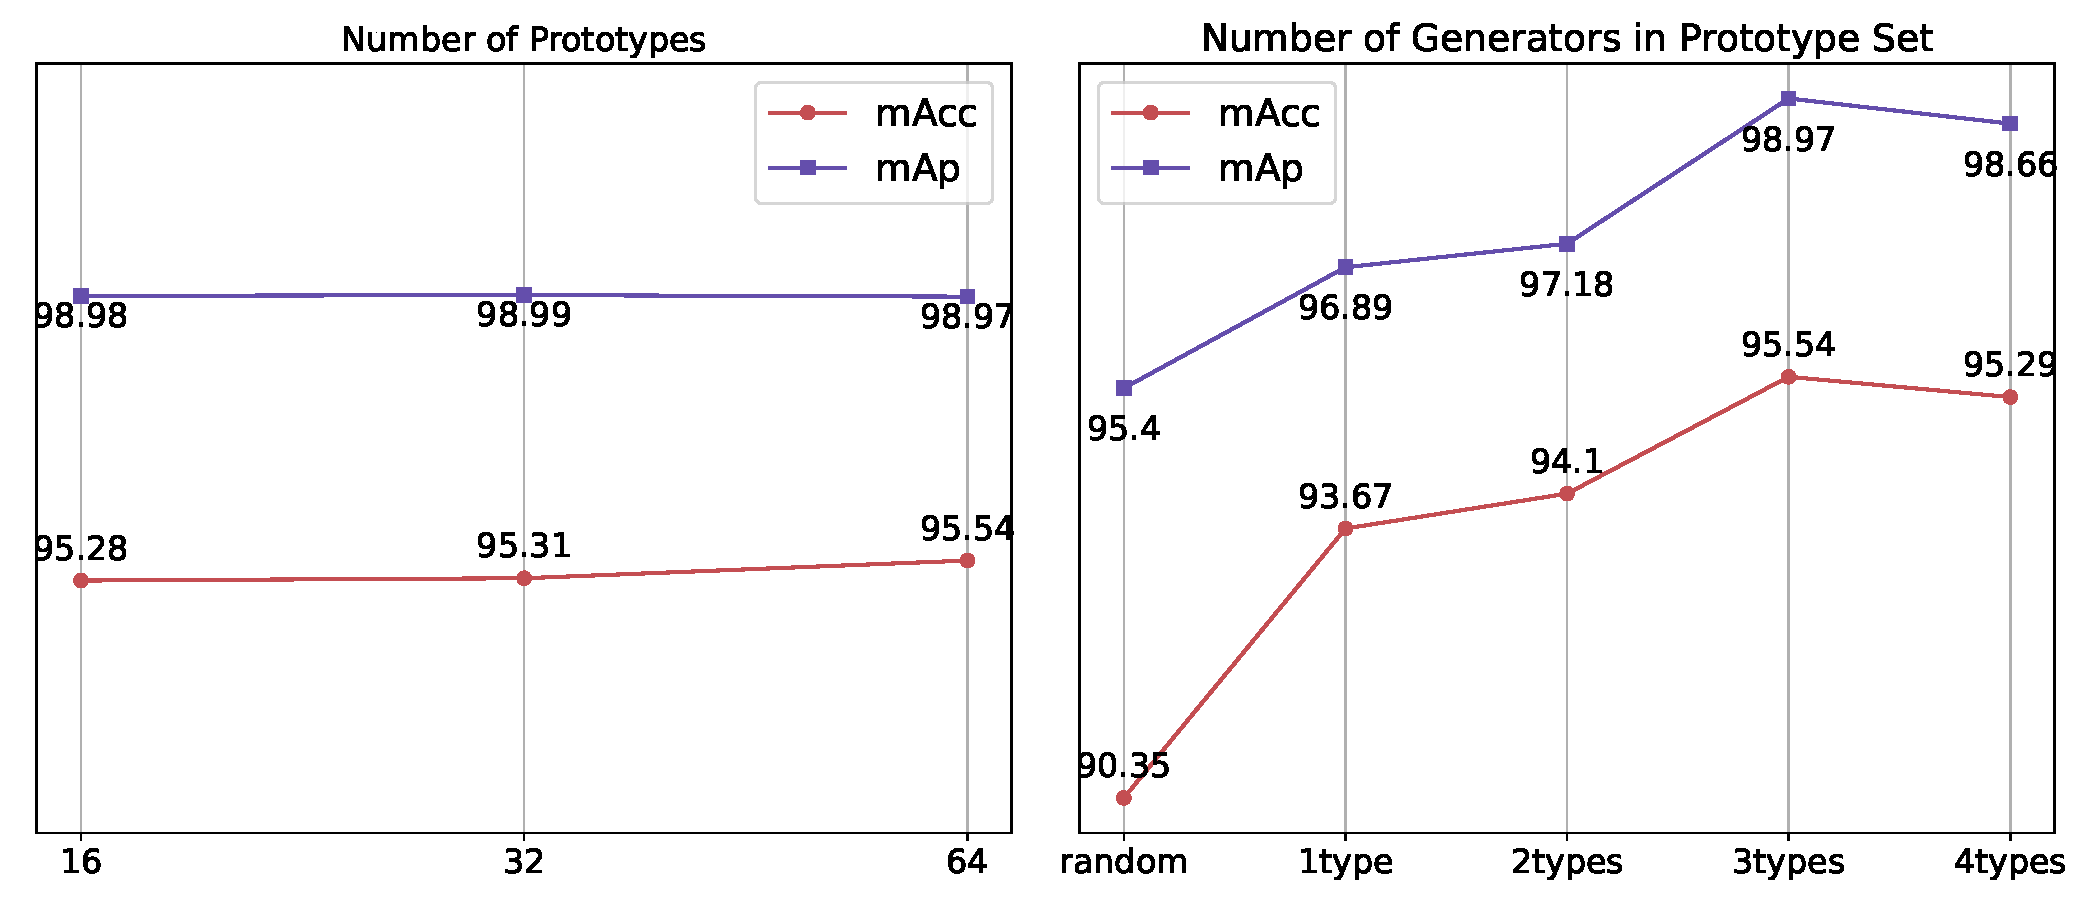
\includegraphics[width=\linewidth]{figs/hyperparam.pdf}
    \caption{Ablation study regarding the strategy of extracting prototypes. We compare number of prototypes retain in PCA and types of generators in Prototype Set. }
    \label{fig:hyperparam}
\end{figure}



% \subsection{Evaluation on robustness (RQ.5)}
        
%     To validate the robustness of our model against post-processing operations, which are commonly encountered in real-world scenarios, we conduct a robustness evaluation on JPEG compression and Gaussian blur.  We select some common AIGI detectors on GenImage dataset as baselines, to align the performance of starting point, we select checkpoints trained on GenImage SD1.4 subset for these baselines. Results in Fig.~\ref{fig:robustness} shows that: \textit{\textbf{(1) GAPL keeps steady performance with minimum degradation}.} The proposed GAPL not only retains the best overall performance but also has an degradation of only 11.09\% and 25.12\% in extreme JPEG compression and gaussian blur. \textit{\textbf{(2) Frequency based AIGI detectors suffer from post process}.} Detectors that leverage frequency domain information like AIDE and SAFE behave bad in JPEG compress experiments, a slight JPEG compression could affect the performance to almost random choice of 50\%. This also suggests that these detectors are unreliable in real life scenarios.

\subsection{Evaluation on robustness (RQ.5)}

    We evaluate robustness under two common post-processing operations, JPEG compression and Gaussian blur. We compare GAPL with representative AIGI detectors on GenImage, using checkpoints trained on the SD1.4 subset to ensure a comparable starting point. Fig.~\ref{fig:robustness} shows that: \textit{\textbf{(1) GAPL remains the most robust.}} It achieves the best overall performance, with only 11.09\% and 25.12\% degradation under extreme JPEG compression and Gaussian blur, respectively. \textit{\textbf{(2) Frequency-based detectors are highly fragile to post-processing.}} Methods such as AIDE and SAFE degrade severely under JPEG compression, with even mild compression reducing performance to near chance level, indicating limited reliability in real-world settings.

\begin{figure}[!t]
    \centering
    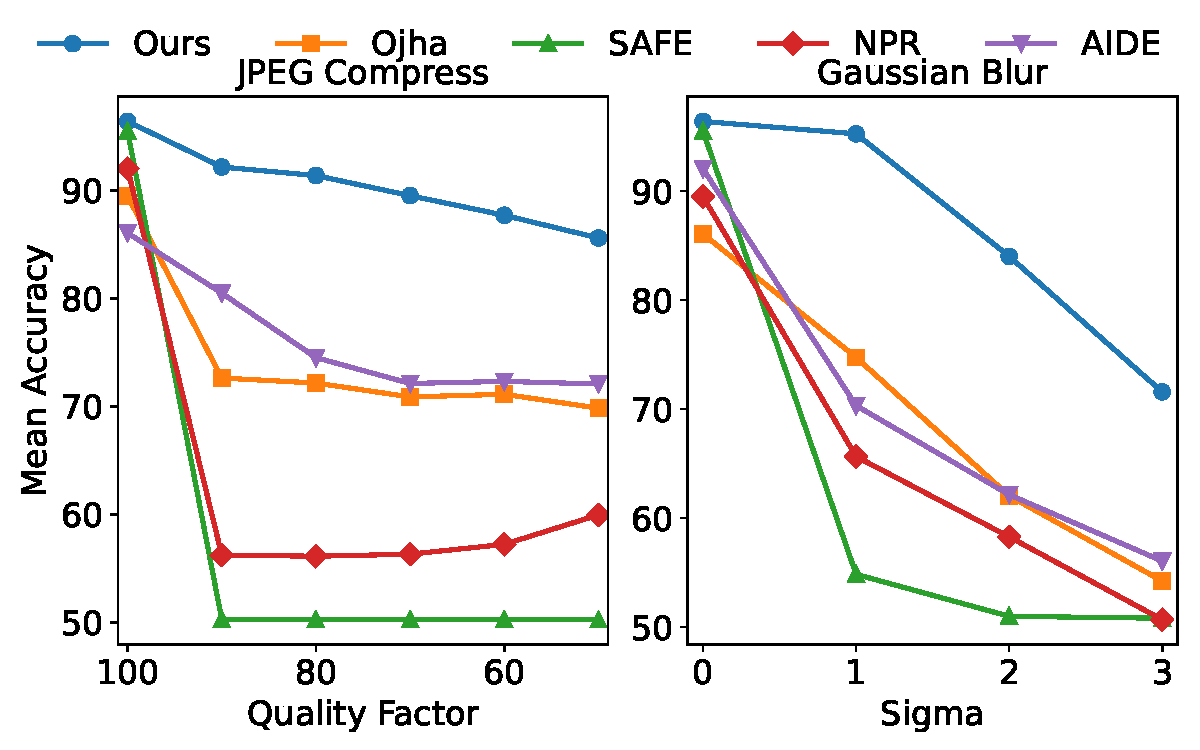
\includegraphics[width=\linewidth]{figs/robustness.pdf}
    \caption{
            Comparison of \textbf{Robustness performance} regarding post process on GenImage dataset. Our model achieve the best overall performance on post process with the minimum degradation.}
        \label{fig:robustness}
\end{figure}

\subsection{Visualization on learned prototypes} 
    To validate \textbf{how our model utilizes prototypes}, we calculate the average attention scores between prototypes and images on the validation set, we plot the results in Fig.~\ref{fig:visualization}. From the figure, \textit{\textbf{(1) certain prototypes are consistently utilized by the model}.} This indicates that some pattern were common in generated images and real images. Subsequently, to uncover what hide behind these frequently utilized prototypes, we clustered the images that exhibited particularly high attention scores for a specific prototype. We find that \textit{\textbf{(2) images pay extreme attention to a certain prototype share some visual characteristics}.} In generated images, those feature distorted objects and unrealistic lines pay high attention to \textit{Prototype \#36}, images pay attention to \textit{Prototype \# 50} usually contain over smooth material surface. As for real images, complex natural scene and consistent portrait light make them look real, which frequently exist in clusters of \textit{Prototype \#4} and \textit{Prototype \#13}. This finding indicates that our method indeed learned some sort of pattern and the mapping between image with these prototypes.
    


\begin{figure}[!t]
        \centering
        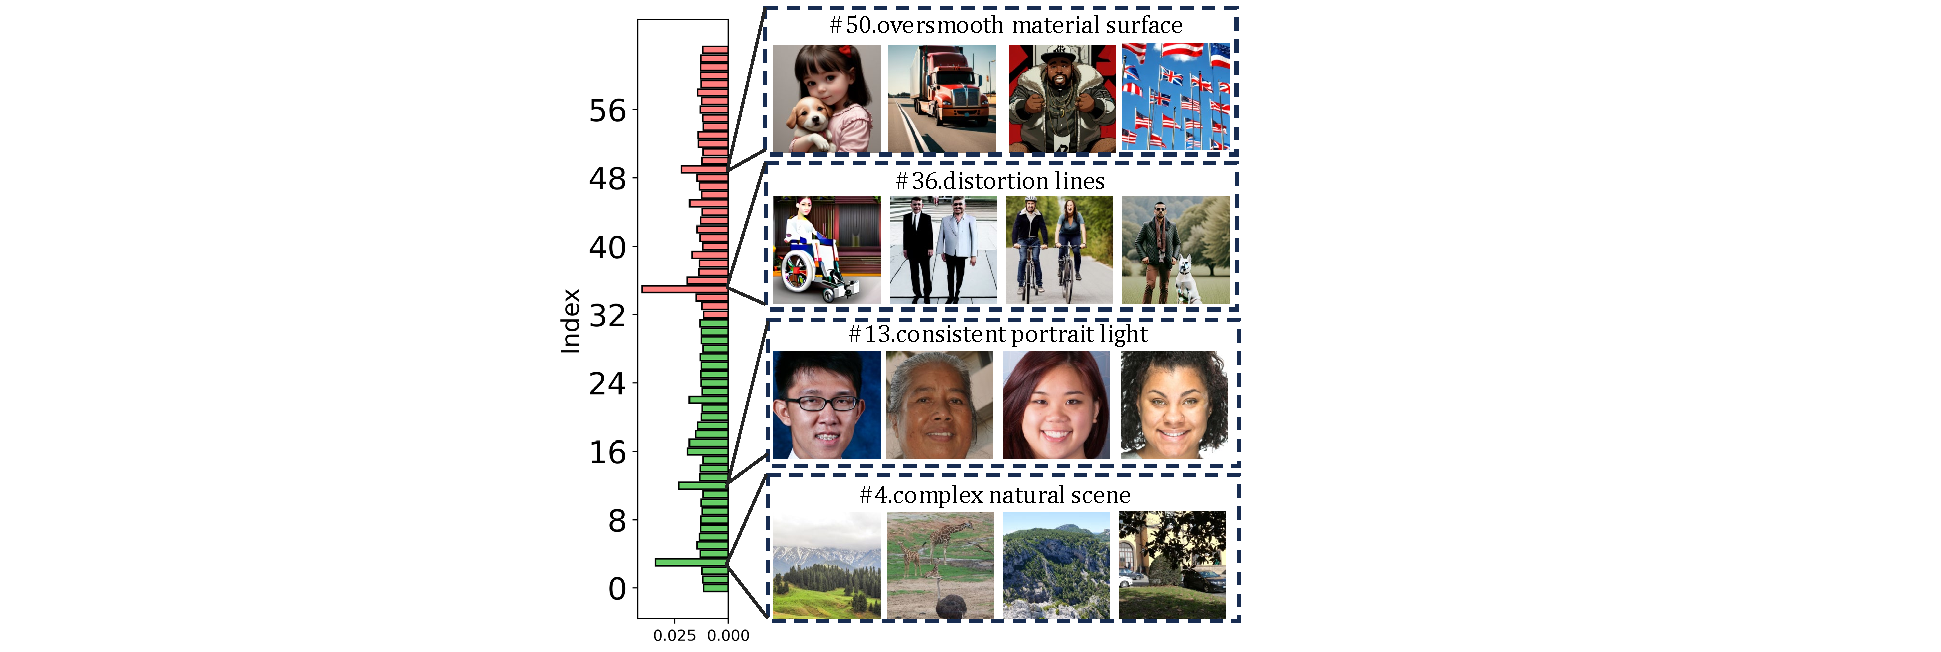
\includegraphics[width=\linewidth]{figs/visual_h.pdf} 
        \caption{
            \textbf{Average attention scores} on the validation set. Column in red and green means prototypes extracted with real images and generated images, respectively. We collected images that exhibit high attention score for a specific prototype and discovered that they have visual features in common.
        }
        \label{fig:visualization} 
\end{figure}


\section{Conclusion}
    In this paper, we study AI-generated image detection in the scaling-up regime. We identify the key challenges of scaling detector training with diverse generators and highlight the limitations of existing methods. To address these issues, we propose GAPL, which is designed to better exploit data from a wide range of generators. Extensive experiments show that scaling up training is essential for building detectors that generalize across diverse generative models, and that GAPL delivers consistent performance under this setting, taking a step toward universal AIGI detection.

    \textbf{Limitation.} Although our method achieves strong and consistent performance on existing benchmarks, its behavior on truly unseen domains remains unclear, especially for future generative models built upon fundamentally new techniques. Whether such models will still leave detectable artifacts, or become increasingly difficult to distinguish from real images, remains an open problem for future research.

\section*{Acknowledgments}
{\raggedright
This work was supported in part by the National Natural Science Foundation of China under Grant 72434005, Grant 72225011 , Grant 72293575, Grant U24B20179 and Grant 62336001.
\par}